\documentclass[tikz,border=8pt]{standalone}
% Shared look for every TikZ diagram. Load with \input{../../tools/tikz-style.tex}
\usepackage[T1]{fontenc}
\usepackage{lmodern}
\renewcommand{\sfdefault}{lmr}  % diagrams use the same serif as the text
\usetikzlibrary{arrows.meta, positioning, shapes.geometric, calc, fit, backgrounds}
\definecolor{cblue}{HTML}{4C78A8}
\definecolor{corange}{HTML}{F58518}
\definecolor{cgreen}{HTML}{54A24B}
\definecolor{cred}{HTML}{E45756}
\definecolor{cpurple}{HTML}{B279A2}
\definecolor{cgrey}{HTML}{6B6B6B}
\tikzset{
  every picture/.style={font=\sffamily, line width=1.2pt},
  box/.style={draw=#1, fill=#1!12, rounded corners=4pt, align=center, inner sep=7pt, minimum height=1.1cm},
  box/.default=cgrey,
  arrow/.style={-{Stealth[length=3mm]}, draw=cgrey, line width=1.4pt},
  title/.style={font=\sffamily\bfseries\Large},
  note/.style={font=\sffamily\small, text=cgrey, align=center},
}
\AtBeginDocument{\hyphenpenalty=10000 \exhyphenpenalty=10000}

% "1 m straight ahead" in the body frame lands at different map points for different headings: (3, 1) facing x, (2, 2) facing y.
\begin{document}
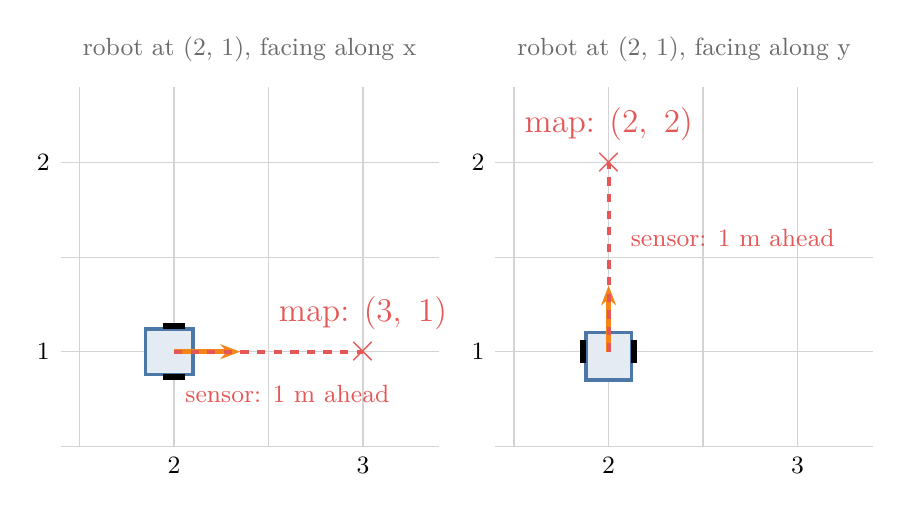
\begin{tikzpicture}[scale=2.4, every node/.append style={font=\large}]
  \foreach \panel/\ang/\ox/\oy/\lab/\sx/\sy/\sa in {0/0/3/1/{facing along x}/2.6/0.88/north, 1/90/2/2/{facing along y}/2.06/1.6/west} {
    \begin{scope}[xshift=\panel*2.3cm]
      \draw[cgrey!30, line width=0.5pt] (1.4,0.5) grid[step=0.5] (3.4,2.4);
      \foreach \t in {2,3} \node[below, font=\small] at (\t,0.5) {\t};
      \foreach \t in {1,2} \node[left, font=\small] at (1.4,\t) {\t};
      \node[note] at (2.4,2.6) {robot at (2, 1), \lab};
      \begin{scope}[shift={(2,1)}, rotate=\ang]
        \draw[cblue, fill=cblue!15] (-0.15,-0.12) rectangle (0.1,0.12);
        \fill[black] (-0.06,0.12) rectangle (0.06,0.15); \fill[black] (-0.06,-0.15) rectangle (0.06,-0.12);
        \draw[-{Stealth[length=2.5mm]}, corange, line width=1.6pt] (0,0) -- (0.35,0);
        \draw[cred, dashed, line width=1.4pt] (0,0) -- (1,0);
      \end{scope}
      \node[cred, font=\small, anchor=\sa] at (\sx,\sy) {sensor: 1 m ahead};
      \node[cred, font=\Large] at (\ox,\oy) {$\times$};
      \node[cred, above=4pt] at (\ox,\oy) {map: $(\ox,\ \oy)$};
    \end{scope}
  }
\end{tikzpicture}
\end{document}
